\chapter{程式碼說明}
\renewcommand{\baselinestretch}{10.0} %設定行距
\pagenumbering{arabic} %設定頁號阿拉伯數字
\setcounter{page}{6}  %設定頁數
\fontsize{14pt}{2.5pt}\sectionef

\section{控制機器人程式}
此控制機器人程式利用 Python 語言。\\
\begin{figure}[hbt!]
\begin{center}
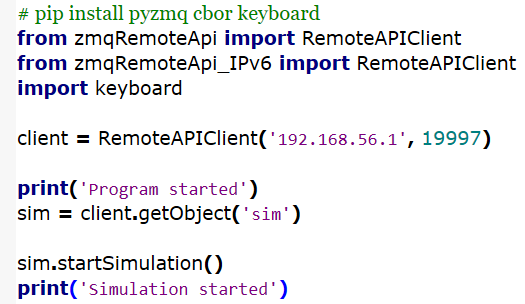
\includegraphics[height=6cm]{bubbleRob code 1}
\caption{\Large 控制機器人程式之一}\label{控制機器人程式之一}
\end{center}
\end{figure} 
使用 pip install pyzmq cbor keyboard 安裝了所需的套件,其中:\\
\begin{itemize}
\item \textbf{pyzmq} 用於建立 ZeroMQ 連線。
\item \textbf{cbor} 用於將資料序列化和反序列化。
\item \textbf{keyboard} 用於操控鍵盤事件。
\end{itemize}
使用 zmqRemoteApi 中的 IPv6  導入了用於建立與 CoppeliaSim 之間通訊的 Remote API 相關程式庫,使得可以通過程式碼控制仿真場景和物件,建立了一個 RemoteAPIClient 物件 client,並將 IP 和埠號分別作為 CoppeliaSim 的 IP 地址和連接埠。\\
這樣就建立了與 CoppeliaSim 的連線,使用 \texttt{client.getObject('sim')} 獲取了 CoppeliaSim 中的 sim 物件,該物件代表了整個仿真環境。透過這個物件,可以執行相關的仿真操作,再來透過  sim.startSimulation() 開始模擬。\\
\newpage

\begin{figure}[hbt!]
\begin{center}
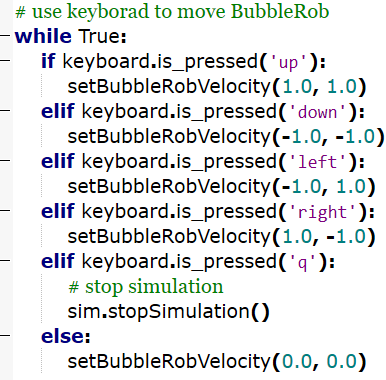
\includegraphics[height=8cm]{bubbleRob code 2}
\caption{\Large 控制機器人程式之二}\label{控制機器人程式之二}
\end{center}
\end{figure} 
這段程式碼是一個無窮迴圈,用於持續感測鍵盤並根據按鍵的狀態來控制機器人的運動。\\
如果按下 'up' 鍵,則呼叫 setBubbleRobVelocity(1.0, 1.0),將機器人的速度設定為正向。\\
如果按下 'down' 鍵,則呼叫 setBubbleRobVelocity(-1.0, -1.0),將機器人的速度設定為反向。\\
如果按下 'left' 鍵,則呼叫 setBubbleRobVelocity(-1.0, 1.0),將機器人的速度設定為左轉。\\
如果按下 'right' 鍵,則呼叫 setBubbleRobVelocity(1.0, -1.0),將機器人的速度設定為右轉。\\
如果按下 'q' 鍵,則停止仿真。若沒有按下上述任何按鍵,則呼叫 setBubbleRobVelocity(0.0, 0.0),將機器人的速度設定為零,即停止移動。\\
\newpage

\section{記分板程式}
此程式是使用 Lua 語言。\\
\begin{figure}[hbt!]
\begin{center}
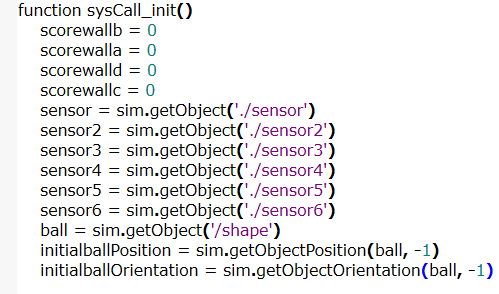
\includegraphics[height=6cm]{scorewall1}
\caption{\Large LED 記分板程式之一}\label{LED 記分板程式之一}
\end{center}
\end{figure} 
設定名稱為 sysCall init 的函數,在程式初始化時被呼叫。該函數的主要目的是初始化一些變數並取得物件的句柄。\\
1. scorewallb = 0、scorewalla = 0、scorewalld = 0、scorewallc = 0 用於初始化四個得分牆的變數,將初始值設為 0。\\
2. \texttt{sim.getObject} 獲取了各感測器及球的句柄。\\
3. \texttt{initialballPosition = sim.getObjectPosition(ball, -1)}:用於取得球體的初始位置。\\
4. \texttt{initialballOrientation = sim.getObjectOrientation(ball, -1)}:用於取得球體的初始方向。\\
\newpage

\begin{figure}[hbt!]
\begin{center}
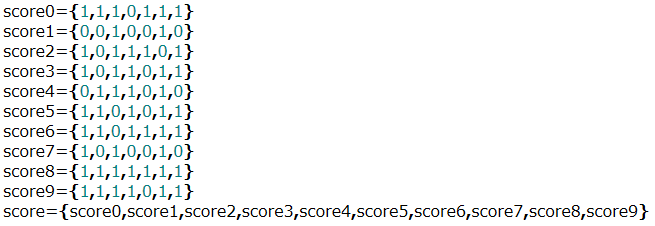
\includegraphics[height=5cm]{scorewall2}
\caption{\Large LED 記分板程式之二}\label{LED 記分板程式之二}
\end{center}
\end{figure} 
定義了一個包含十個元素的表格,每個元素都是由七個二進制數字(0或1)組成的列表。每個列表代表一個數字(0到9)的數字模式,而最後一行程式碼將這些數字模式放入一個名為 score 的表格中,以便在程式中進行使用。\\
\newpage

\begin{figure}[hbt!]
\begin{center}
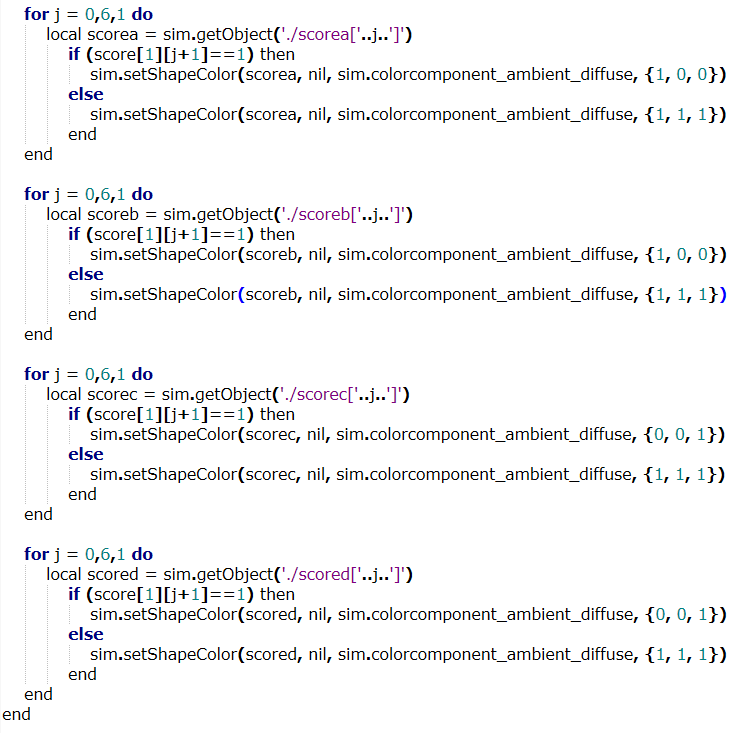
\includegraphics[height=10cm]{scorewall3}
\caption{\Large LED 記分板程式之三}\label{LED 記分板程式之三}
\end{center}
\end{figure}
這段程式碼是一個迴圈,用於對記分板進行顏色設定,根據事先定義的數字模式進行,迴圈的運行範圍是從0到6每次遞增1,在迴圈的每次迭代中,會執行以下操作:\\
1. scorewallb = 0、scorewalla = 0、scorewalld = 0、scorewallc = 0 用於初始化四個得分牆的變數,將初始值設為 0。\\
2. 創建一個指向記分板的參考是由迴圈變量 j 指定。\\
3. 檢查表格中的特定位置如果該位置的值等於 1,則使用 \texttt{sim.setShapeColor}函數設定記分板數字的顏色為紅色。\\
4. 如果該位置的值不等於 1,使用 \texttt{sim.setShapeColor}函數設定記分板數字的顏色為白色。\\
\newpage

\begin{figure}[hbt!]
\begin{center}
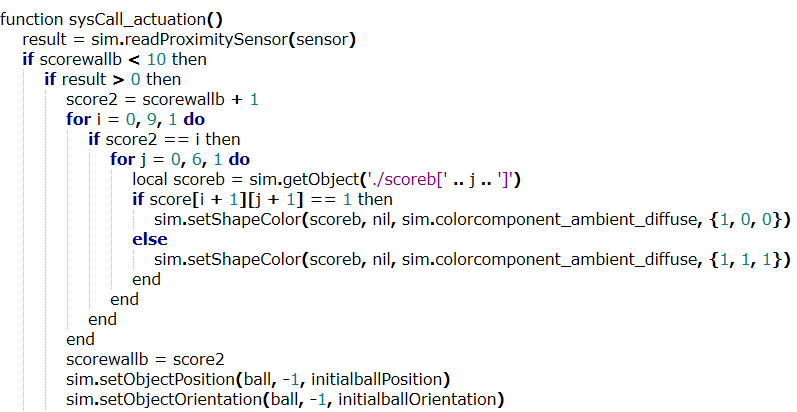
\includegraphics[height=8cm]{scorewall4}
\caption{\Large LED 記分板程式之四}\label{LED 記分板程式之四}
\end{center}
\end{figure} 
在此函式中,首先使用 \texttt{sim.readProximitySensor}函式讀取 sensor 的近接傳感器數值,並將結果存儲在 result 變數中,如果 scorewallb 小於 10,且如果 result 大於 0,表示與某個物體接觸。則執行以下操作:\\
1. 將 score2 設定為 scorewallb 加 1。\\
2. 進行一個迴圈從 0 到 9,每次遞增 1。\\
3. 如果 score2 等於 i 進行另一個迴圈從 0 到 6 每次遞增 1,創建一個指向 scoreb 的參考由迴圈 j 變量檢查 score 表格中的特定位置,如果該位置的值等於 1 使用 \texttt{sim.setShapeColor}函式設定 scoreb 物體的顏色為紅色,如果該位置的值不等於 1 使用 \texttt{sim.setShapeColor}函式設定 scoreb 物體的顏色為白色。\\
4. 更新 scorewallb 的值為 score2。\\
5. 使用 \texttt{sim.setObjectPosition} 函式將 ball 物體的位置設定為初始位置。\\
6. 使用 \texttt{sim.setObjectOrientation} 函式將 ball 物體的方向設定為初始方向。\\
\newpage

\begin{figure}[hbt!]
\begin{center}
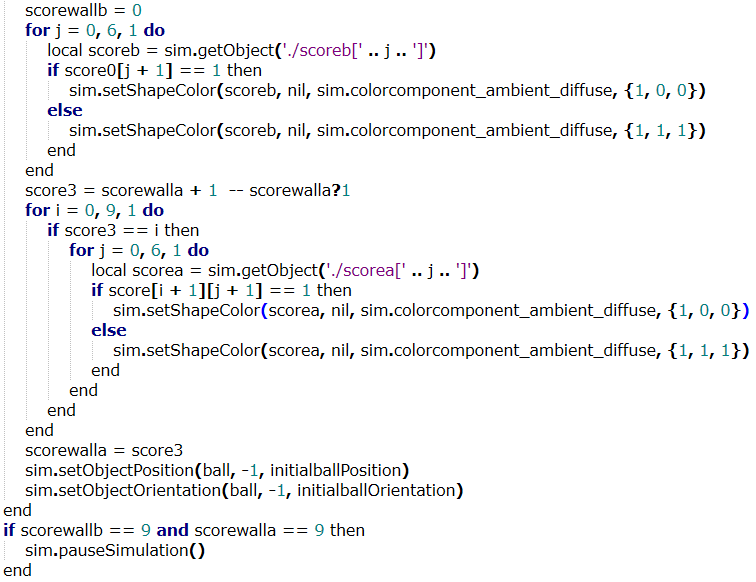
\includegraphics[height=10cm]{scorewall5}
\caption{\Large LED 記分板程式之五}\label{LED 記分板程式之五}
\end{center}
\end{figure} 
反之如果 scorewallb 大於 9 則執行以下操作:\\
1. 將 scorewallb 的值設定為 0。\\
2. 進行一個迴圈從 0 到 6,每次遞增 1 創建一個指向 scoreb 物體的參考,該物體是由迴圈變量 j 指定的物體,如果該位置的值等於 1 使用 \texttt{sim.setShapeColor}函式設定 scoreb 物體的顏色為紅色,如果該位置的值不等於 1 使用 \texttt{sim.setShapeColor}函式設定 scoreb 物體的顏色為白色。\\
3. 將 score3 設定為 scorewalla 加 1。\\
4. 更新 scorewallb 的值為 score2。\\
5. 進行一個迴圈從 0 到 9,每次遞增 1 ,如果 score3 等於 i 進行一個迴圈從 0 到 6,每次遞增 1 創建一個指向 scoreb 物體的參考,該物體是由迴圈變量 j 指定的物體,如果該位置的值等於 1 使用 \texttt{sim.setShapeColor}函式設定 scoreb 物體的顏色為紅色,如果該位置的值不等於 1 使用 \texttt{sim.setShapeColor}函式設定 scoreb 物體的顏色為白色。\\
6. 更新 scorewalla 的值為 score3。\\
7. 使用 \texttt{sim.setObjectPosition} 函式將 ball 物體的位置設定為初始位置。\\
8. 使用 \texttt{sim.setObjectOrientation} 函式將 ball 物體的方向設定為初始方向。\\
9. 程式碼檢查兩個變數 scorewallb 和 scorewalla 是否都等於 9。如果兩個變數的值都等於 9 用  \texttt{sim.pauseSimulation()} 函式暫停仿真。\\
而另一隊記分板也是使用一樣的程式只是更改名稱。\\

\begin{figure}[hbt!]
\begin{center}
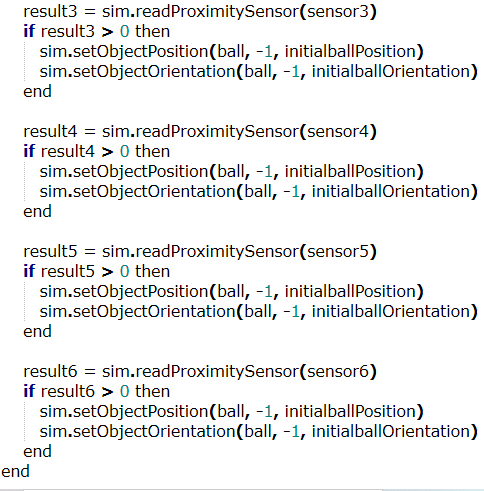
\includegraphics[height=8cm]{scorewall6}
\caption{\Large LED 記分板程式之六}\label{LED 記分板程式之六}
\end{center}
\end{figure} 
如果感測器感測到物體則執行以下操作:\\
1. 使用 \texttt{sim.setObjectPosition} 函式將 ball 物體的位置設定為初始位置。\\
2. 使用 \texttt{sim.setObjectOrientation} 函式將 ball 物體的方向設定為初始方向。\\
\newpage

\begin{figure}[hbt!]
\begin{center}
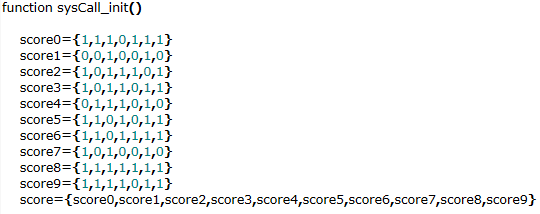
\includegraphics[height=8cm]{time1}
\caption{\Large 計時器程式之一}\label{計時器程式之一}
\end{center}
\end{figure} 
沿用了記分板的程式:\\
設定名稱為 sysCall init 的函數,在程式初始化時被呼叫。該函數的主要目的是初始化一些變數並取得物件的句柄。\\定義了一個包含十個元素的表格,每個元素都是由七個二進制數字(0或1)組成的列表。每個列表代表一個數字(0到9)的數字模式,而最後一行程式碼將這些數字模式放入一個名為 score 的表格中,以便在程式中進行使用。\\
\newpage

\begin{figure}[hbt!]
\begin{center}
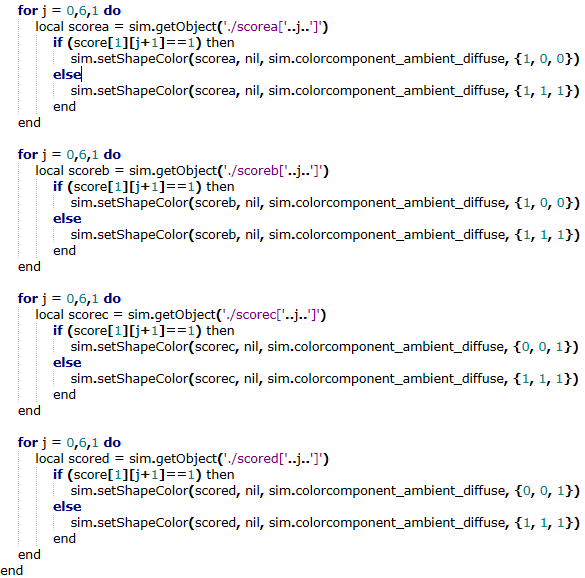
\includegraphics[height=8cm]{time2}
\caption{\Large 計時器程式之二}\label{計時器程式之二}
\end{center}
\end{figure} 
沿用了記分板的程式:\\
這段程式碼是一個迴圈,用於對記分板進行顏色設定,根據事先定義的數字模式進行,迴圈的運行範圍是從0到6每次遞增1,在迴圈的每次迭代中,會執行以下操作:\\
1. scorewallb = 0、scorewalla = 0、scorewalld = 0、scorewallc = 0 用於初始化四個得分牆的變數,將初始值設為 0。\\
2. 創建一個指向記分板的參考是由迴圈變量 j 指定。\\
3. 檢查表格中的特定位置如果該位置的值等於 1,則使用 \texttt{sim.setShapeColor}函數設定記分板數字的顏色為紅色。\\
4. 如果該位置的值不等於 1,使用 \texttt{sim.setShapeColor}函數設定記分板數字的顏色為白色。\\
\newpage

\begin{figure}[hbt!]
\begin{center}
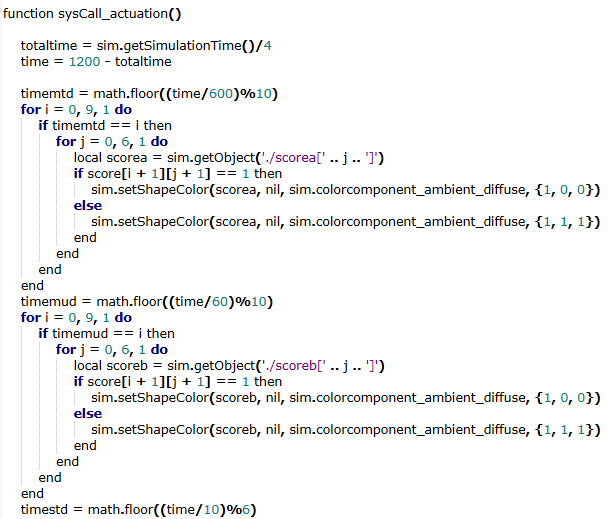
\includegraphics[height=8cm]{time3}
\caption{\Large 計時器程式之三}\label{計時器程式之三}
\end{center}
\end{figure} 
1. totaltime = \texttt{sim.getSimulationTime()/4}: 計算從模擬開始到現在的總時間,並除以 4(為了調整時間的比例)。\\
2. \texttt{time = 1200 - totaltime}:根據總時間計算剩餘時間,1200 這部分可依照自己需求去修改。\\
3. \texttt{timemtd = math.floor((time/600)\%10):根據剩餘時間計算十位數分鐘數字,math.floor 函數用於將計算結果向下取整,\% 表示取模運算符號,這裡是將時間除以 600 取其餘數,再取該餘數的整數部分。\\
4. \texttt{for i = 0, 9, 1 do}:進行一個迴圈從 0 到 9,每次遞增 1。\\
5. \texttt{if timemtd == i then}:檢查十位數分鐘是否等於當前迴圈數字。\\
6. 在內部循環 \texttt{for j = 0, 6, 1 do} 中,進行顯示相關的操作。\\
7. \texttt{local scorea = sim.getObject('./scorea[' .. j .. ']')}:獲取記分板十位數分鐘的句柄。\\
8. \texttt{if score[i + 1][j + 1] == 1 then}:檢查特定位置上的數字是否為 1(即該位置需要亮起)。\\
9. \texttt{sim.setShapeColor(scorea, nil, sim.colorcomponent_ambient_diffuse, {1, 0, 0})}:設置該顯示元素的顏色為紅色(表示亮起)。\\
10. \texttt{sim.setShapeColor(scorea, nil, sim.colorcomponent_ambient_diffuse, {1, 1, 1})}:設置該顯示元素的顏色為白色(表示熄滅)。\\
11. \texttt{timemtd = math.floor ((time/60)\%600)}:分別用於計算十位數分鐘數字,並根據結果進行相應的顯示操作。\\
個位數分鐘與上面程式相同唯一不同的是 \texttt{timemud = math.floor((time/10)\%60)}用於計算個位數分鐘數字,並根據結果進行相應的顯示操作。\\
\newpage

\begin{figure}[hbt!]
\begin{center}
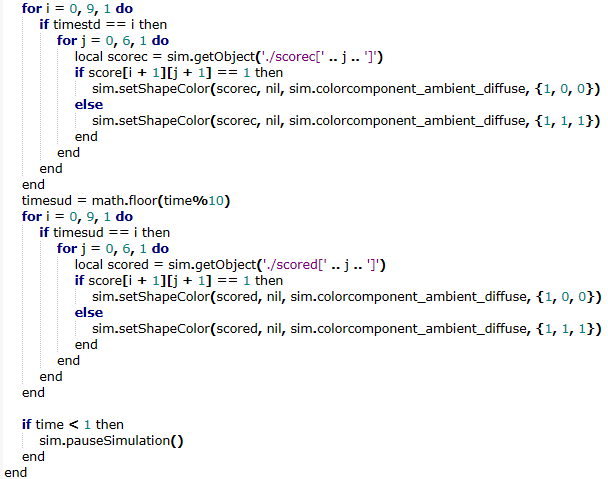
\includegraphics[height=8cm]{time4}
\caption{\Large 計時器程式之四}\label{計時器程式之四}
\end{center}
\end{figure} 
程式與十位、個位數分鐘相同唯一不同的是 
1. \texttt{timestd = math.floor((time/10)\%10)} 用於計算十位數秒鐘數字,並根據結果進行相應的顯示操作。\\
2. \texttt{timesud = math.floor(time/10)} 用於計算個位數秒鐘數字,並根據結果進行相應的顯示操作。\\
3. 當時間小於 1 時停止模擬。\\
\newpage
\renewcommand{\baselinestretch}{1.0} %設定行距